\documentclass[12pt,a4paper,titlepage,twoside]{report}
\usepackage[utf8]{inputenc}
\usepackage[french]{babel}
\usepackage[T1]{fontenc}
\usepackage{amsmath}
\usepackage{amsfonts}
\usepackage{amssymb}
\usepackage{graphicx}
\usepackage{url}
\usepackage[usenames,dvipsnames]{xcolor}
\usepackage[colorlinks=false,urlbordercolor=white,linkbordercolor=white]{hyperref}
\usepackage[left=2cm,right=2cm,top=2cm,bottom=2cm]{geometry}
\usepackage{fancyhdr}
\usepackage{lmodern}
\usepackage{listings}
\pagestyle{fancy}
\usepackage{titlesec}
\usepackage[abs]{overpic}
\usepackage{hyperref}
\usepackage{pdfpages}

% Definition des couleurs
\definecolor{titreColor}{RGB}{0,58,128}  % Marine
\definecolor{stitreColor}{RGB}{0,158,224}  % Ocean
\definecolor{auteurColor}{RGB}{0,58,128}     % Marine
\definecolor{texteColor}{RGB}{164,196,0}     % Prairie

% Definition des chapitres
\titleformat{\chapter}[display]
{\normalfont\Large\filcenter\sffamily}
{\titlerule[1pt]%
 \vspace{1pt}%
 \titlerule
 \vspace{1pc}%
 \Large\color{titreColor}{\chaptertitlename} \thechapter}
{1pc}
{\titlerule
 \vspace{1pc}%
 \Huge}

\titleformat{\section}
{\color{titreColor}\normalfont\Large\bfseries\sffamily}
{\color{titreColor}\thesection}{1em}{}

\titleformat{\subsection}
{\color{stitreColor}\bfseries\sffamily}
{\color{stitreColor}\thesubsection}{1em}{}

%Données de titre et d'auteur pour la page de garde
\newcommand{\titre}{Logiciel ALISMA}
\newcommand{\sousTitre}{Manuel d'installation et d'utilisation}
\newcommand{\auteur}{Irstea -- centre de Bordeaux}
\newcommand{\dateModif}{Version 1.2 du x mars 2018}

\begin{document}
%Supprime les veuves et orphelines
\widowpenalty=10000
\clubpenalty=10000
\raggedbottom 

% Integre la page de garde
%\setcounter{page}{0}
\thispagestyle{empty}
% Logo IRSTEA
\vspace{-2cm}
\hspace{-2cm}

\includegraphics[width=3.06cm,height=3.06cm,keepaspectratio]{logo_irstea}%


\vspace*{4cm}
\hspace{5cm}
\setlength\unitlength{1mm}
% Logo de titre
\begin{overpic}[width=9.44cm,height=9.57cm,keepaspectratio]{logo_fond_droite.png}
% Titre du document
\put(-50,50){
\begin{minipage}{0.7\linewidth}
\Huge\flushright \color{titreColor}{\bfseries\sffamily\titre{}}\\
% sous-titre du document
\color{stitreColor}{\Large \bfseries\sffamily\sousTitre{}}
\end{minipage}
}
\end{overpic}

%  date et auteur
% creation de l'espace a gauche
\vspace*{1cm}
\begin{minipage}{0.5\linewidth}
\hfill
\end{minipage}
% positionnement
\begin{minipage}{0.5\linewidth}\flushleft{
% Date
\textcolor{auteurColor}{\Large\sffamily\dateModif{}}\\
\vspace*{0.1cm}
% Auteur
\textcolor{auteurColor}{\Large\sffamily\auteur{}}\\
\vspace{0.5cm}
% Adresse
\textcolor{texteColor}{\sffamily\textbf{IRSTEA} - Centre de Bordeaux\\
50, avenue de Verdun, Gazinet\\
33612 CESTAS Cedex }
}
\end{minipage}
% Ligne de logos
\begin{minipage}{\linewidth}

% logos complémentaires
%\vspace{3cm}
%\hspace{2cm}
%\includegraphics[width=3cm,height=3cm,keepaspectratio]
%{emplacement_logo}%
%\vspace{-1cm}
%\hspace{1cm}
%\includegraphics[width=3cm,height=3cm,keepaspectratio]
%{emplacement_logo}%
%\vspace{-1cm}
%\hspace{1cm}
%\includegraphics[width=3cm,height=3cm,keepaspectratio]
%{emplacement_logo}%
\end{minipage}
% Définition des entêtes
\fancyhead{}
\fancyhead[CO]{\leftmark\sffamily}
\fancyhead[CE]{ \sffamily\titre{}}
\fancyfoot[CO]{\sffamily\thepage}
\fancyfoot[CE]{\sffamily\thepage}
% Redéfinition de \cleardoublepage pour créer une page vide
\makeatletter
\def\cleardoublepage{\clearpage\if@twoside \ifodd\c@page\else
  \hbox{}
  \vspace*{\fill}

  \vspace{\fill}
  \thispagestyle{empty}
  \newpage
  \if@twocolumn\hbox{}\newpage\fi\fi\fi}
\makeatother

% \cleardoublepage permet de générer une page vide 
% si le chapitre ne commence pas sur la page de droite
%\cleardoublepage
\chapter{Introduction}

\section{Objectifs du logiciel}
Le logiciel ALISMA est conçu pour permettre la saisie des relevés des macrophytes réalisés en cours d'eau, dans le cadre de la DCE \og Cours d'eau \fg{}. 

Il permet le calcul de l'indicateur.

Pour toutes informations concernant le protocole, consultez le site \href{https://hydrobio-dce.irstea.fr/cours-deau/macrophytes/}{hydrobio-dce.irstea.fr/cours-deau/macrophytes/}

\subsection{Technologie employée}
Le logiciel a été écrit en Java. Il fonctionne soit en mode \textit{monoposte} avec une base de données embarquée HSQLDB (fonctionnement transparent pour l'utilisateur), soit en mode réseau, avec une base de données MySQL, pour un partage des informations entre plusieurs utilisateurs.

\subsection{Clauses de propriété}
Le logiciel est distribué sous la licence GNU GPL v3 (\url{http://www.gnu.org/licenses/gpl.txt}).

La version 1.0 a été déposée à l'Agence de Protection des Programmes (\url{https://www.app.asso.fr}), sous le numéro \textbf{IDDN.FR.001.270035.000.S.C.2016.000.31500}

\section{Assistance et maintenance}

\subsection{Limite de responsabilité - sécurité}

Le logiciel est fourni \textit{en l'état}, il ne peut être fait grief à Irstea d'un quelconque problème, d'une perte ou d'une corruption des données, ou d'un dysfonctionnement.

Il appartient à l'organisme utilisateur d'assurer la sécurité de ses données tant en confidentialité qu'en intégrité ou en disponibilité, selon les besoins de sécurité qu'il aura déterminé. 

Selon le mode de fonctionnement, il devra soit réaliser une copie du dossier contenant la base de données (mode autonome -- HSQLDB) soit s'assurer que les sauvegardes sont correctement réalisées et recopier les fichiers générés sur un support tiers (mode réseau -- MySQL).

En particulier, même si l'application propose une fonction de sauvegarde de la base de données qui est activée régulièrement, il appartient à l'utilisateur de vérifier qu'elle s'exécute correctement. Il devra également la copier vers un support protégé pour éviter tout risque de perte accidentelle.

\subsection{Dysfonctionnement du logiciel}

En cas de dysfonctionnement de l'application, il est possible d'ouvrir un ticket dans \textit{github}, à l'adresse \url{https://github.com/Irstea/alisma/issues/new}.

Irstea ne prend pas d'engagement concernant leur traitement ou leur prise en compte.

\section{Description des versions}
Le détail des versions est décrit dans le fichier \textit{news.txt}, présent à la racine de l'application.


%\section{Première section}
%\subsection{sous-section}
%Exemple de texte
%\subsection{autre sous-section}

% Second chapitre
%\cleardoublepage
\chapter{Installer le logiciel}

\section{Installer les pré-requis}
\subsection{JRE Java}
Si nécessaire (votre ordinateur dispose peut-être déjà d'une version du JRE), téléchargez le programme d'installation du JRE Java à partir du site : \url{http://www.oracle.com/technetwork/java/javase/downloads/jre7-downloads-1880261.html}
\subsection{Serveur MySql}
Le serveur MySql est utilisé pour gérer les données de l'application.

Vous avez besoin d'installer un serveur MySql dans votre poste de travail si vous voulez que votre application fonctionne de manière autonome. Si vous disposez d'un serveur, installez plutôt MySql dans le serveur ; vous n'aurez alors besoin de n'installer qu'un client pour exécuter les scripts de création et de pré-remplissage de la base de données.

Consultez le cas échéant votre correspondant informatique pour savoir quelle est la meilleure stratégie à adopter.

Pour télécharger MySQL serveur : \url{http://dev.mysql.com/downloads/windows/installer/}

\subsubsection{Configurer le serveur MySql}
Dans le dossier d'installation de MySql, ouvrez le fichier \textit{my.cnf} ou \textit{my.ini} (en principe, dans le dossier : C:\textbackslash{} ProgramData\textbackslash{}MySQL\textbackslash{}MySQL Server 5.6. Dans la section [mysqld], recherchez l'entrée \textit{max\_allowed\_packet}, et vérifiez que la valeur soit au minimum à 16M :
\begin{lstlisting}
[mysqld]
...
max_allowed_packet      = 16M
\end{lstlisting}

Dans le cas contraire, l'import des données de référence (table des stations ou des espèces, notamment) risque de ne pas aboutir.

Relancez ensuite le serveur Mysql.

\subsection{Client MySql}
Le programme sait se connecter directement au serveur MySql, sans passer par des outils tiers. Vous n'avez besoin d'un client, par exemple SQL Workbench, uniquement pour exécuter les scripts de création et de remplissage de la base de données.

Pour télécharger SqlWorkbench : \url{http://dev.mysql.com/downloads/workbench/}


\section{Installer le logiciel}
\subsection{Créer le dossier d'installation}

Le logiciel peut être installé à n'importe quel endroit dans le micro-ordinateur. Néanmoins, privilégiez l'installation soit dans le dossier \textit{program\textbackslash alisma}, soit directement dans un dossier à la racine de votre disque, par exemple \textit{c:\textbackslash alisma}.

\subsection{Décompresser l'archive}
Décompressez le fichier \textit{alisma.zip} dans le dossier d'installation. Vous devriez récupérer la structure suivante :

\begin{itemize}
\item Dossiers :
\begin{description}
\item[database] : scripts d'installation de la base de données ;
\item[param] : contient le fichier de paramètres ;
\item[license] : contient les fichiers de licence d'utilisation du logiciel ;
\item[alisma\_lib] : bibliothèques complémentaires utilisées par l'application.
\end{description}
\item fichiers :
\begin{description}
\item[alisma.jar] : fichier contenant le programme java ;
\item[alisma.bat] : programme de lancement à partir de Windows ;
\item[alisma.sh] : programme de lancement à partir de Linux ;
\item[alisma.png] : icône de l'application, pour créer un raccourci, par exemple (ce fichier n'est pas utilisé directement dans l'application) ;
\item[langage.config] : fichier créé à la première utilisation, qui contient la langue utilisée par défaut.
\end{description}
\end{itemize}

\section{Créer la base de données}
Connectez-vous à votre serveur MySQL, avec les droits vous permettant de créer une base de données.

Si vous avez installé le serveur MySQL localement (dans votre ordinateur), utilisez ces informations :
\begin{description}
\item[serveur] : \textit{localhost}
\item[login] : \textit{root}
\item[password] : laisser à vide\footnote{Les dernières versions de MySql imposent l'utilisation d'un mot de passe pour le compte root}
\end{description}

Créez la base de données (ou \textit{schéma}, dans la terminologie MySql) \textbf{alisma}, associée au login \textbf{alisma} et au mot de passe \textbf{alisma} (paramètres par défaut dans le fichier de configuration).

Les scripts de création et d'alimentation de la base de données sont stockés dans le dossier \textit{database}. Ils doivent être exécutés dans cet ordre, sous peine de déclencher des messages d'erreur de cohérence :
\begin{enumerate}
\item \textit{create\_alisma\_v1.0.sql} : script de création de la base de données \textit{alisma} ;
\item \textit{parametre\_populate\_v1.0.sql} : import des paramètres généraux ;
\item \textit{taxons\_populate\_v1.0.sql} : import du référentiel IRSTEA ;
\item \textit{cours\_eau\_populate\_v1.0.sql} : import des cours d'eau déclarés dans les stations du référentiel SANDRE ;
\item \textit{stations\_populate\_v1.0.sql} : import des stations du référentiel SANDRE.
\end{enumerate}

\subsection{Appliquer les mises à jour}

Si la version du script de création est antérieure à la version de l'application, il est possible qu'il soit nécessaire d'appliquer un script de modification.

Consultez le chapitre \ref{dbmaj} \textit{\nameref{dbmaj}}, page \pageref{dbmaj} pour plus de détails sur la numérotation des scripts de mise à jour.

\section{Adapter les paramètres à votre installation}
\label{sec:param}
Le fichier \textit{param\textbackslash{}param.ini} contient les paramètres qui peuvent être modifiés facilement par l'utilisateur. Néanmoins, la plus grande prudence est de mise, le risque de créer des dysfonctionnements ultérieurement n'étant alors pas nul...

Pour modifier le fichier \textit{param.ini}, utilisez \textit{notepad++} (\url{https://notepad-plus-plus.org}) plutôt que \textit{notepad}, pour éviter les problèmes de caractères de fin de ligne, qui sont différents entre Windows et les autres systèmes d'exploitation.

Le fichier de paramètres est organisé en sections :

\subsection{database}
Cette section précise les paramètres de connexion à la base de données (entre parenthèses, les valeurs par défaut).
\begin{description}
\item [server] : nom du serveur (\textit{localhost})
\item [dbname] : nom de la base de données (\textit{alisma})
\item [dbuser] : nom du compte de connexion (\textit{alisma})
\item [dbpass] : mot de passe de connexion (\textit{alisma})
\item [jdbc\_class] : nom du pilote d'accès à la base de données (\textit{com.mysql.jdbc.Driver})
\item [dbtype] : type de la base de données (\textit{mysql})
\item [backupFileNamePrefix] : préfixe utilisé pour les sauvegardes de la base de données (\textit{alisma\_db})
\item [backupProgram] : nom du programme utilisé pour réaliser la sauvegarde de la base de données (\textit{c:\textbackslash{}Program Files\textbackslash{}MySQL\textbackslash{}MYSQL Server 5.6\textbackslash{}bin\textbackslash{}mysqldump.exe})
\item [pathFolderDataSave] : chemin de stockage des sauvegardes (\textit{c:\textbackslash{}alisma\textbackslash{}backup})
\item [pathFileDateSave] : chemin d'accès au fichier contenant la date de la dernière sauvegarde réalisée (\textit{c:\textbackslash{}alisma\textbackslash{}backup\textbackslash{}alisma\_save.txt})
\item [backupDelay] : délai entre deux sauvegardes (7). Pour inhiber la réalisation des sauvegardes, ce paramètre doit être positionné à \textbf{-1}
\end{description}

Si votre base de données est hébergée dans un serveur, contactez votre administrateur informatique pour connaître les paramètres à renseigner.

\subsection{language}

Cette section permet de définir la langue utilisée par défaut dans le logiciel.

\begin{description}
\item [default] : langue utilisée par défaut (fr\_FR)
\item [preferred] : langue préférée (fr\_FR)
\item[en\_US]: langue utilisée en cas de libellé manquant (fr\_FR)
\item [en\_EN] : idem
\end{description}


\subsection{others}

\begin{description}
\item [modeDebug] : active l'affichage des messages dans le logiciel (false)
\item [lambert] : indique si les coordonnées Lambert sont utilisées (true). Si le logiciel est employé pour des relevés hors France, basculez ce paramètre à \textbf{false}
\item [lambert93Emin] : coordonnée Lambert Est minimale (70000)
\item [lambert93Emax] : coordonnée Lambert Est maximale (1200000)
\item [lambert93Nmin] : coordonnée Lambert Nord minimale (6000000)
\item [lambert93Nmax] : coordonnée Lambert Nord maximale (7200000)
\item [pathFolderExport] : chemin de stockage des fichiers générés (c:\textbackslash{}alisma\textbackslash{}export)
\item [exportFileNamePrefix] : préfixe utilisé pour les fichiers exportés (alisma)
\item [xsltfile\_fr] : nom du fichier contenant le filtre utilisé pour générer les fichiers PDF, en français (param/alisma.xsl)
\item [xsltfile\_en] : nom du fichier contenant le filtre utilisé pour générer les fichiers PDF, en anglais (param/alisma.xsl)

\end{description}

\subsection{fieldslevel}
Cette section permet de rendre certains champs obligatoires ou non. Quatre niveaux sont disponibles :
\begin{itemize}
\item \textit{vide} : pas de contrôle particulier sur le champ ;
\item \textit{recommanded} : le champ concerné devrait être renseigné ;
\item \textit{necessary} : le champ doit être renseigné pour que le dossier soit validé ;
\item \textit{mandatory} : le champ doit être renseigné pour pouvoir enregistrer le dossier.
\end{itemize}

Dans la pratique, ces niveaux ne sont modifiables que pour les informations suivantes :
\begin{description}
\item [coord\_x et coord\_y] : coordonnées Lambert. Les valeurs doivent être vidées si le logiciel est utilisé hors de France (modification à réaliser en même temps pour le paramètre \textit{others/lambert}) 
\item [wgs84\_x et wgs84\_y] : coordonnées WGS84 (recommanded).
\end{description}

\subsection{display}
Cette section contient le code des couleurs employées, ainsi que les adresses des logos.
\begin{description}
\item [colorFooter] : couleur du bas d'écran (150,182,254)
\item [colorBanniere] : couleur de la bannière (150,182,254)
\item [colorCentral] : couleur de la fenêtre (157,212,255)
\item [colorTab] : couleur des onglets (0,20,205)
\item [icone] : nom du fichier contenant l'icône de l'application (ressources/alisma.png)
\item [logo] : nom du fichier contenant le logo d'IRSTEA (ressources/logo.png)
\end{description}

\section{Mettre à jour le logiciel}
\label{maj}
Lors de la livraison d'une nouvelle version, voici les opérations à réaliser.

Lisez le fichier \textit{news.txt} ou \textit{lisezmoi.txt}, qui peuvent contenir des informations complémentaires nécessaires pour la mise à jour.

\subsection{Installer la nouvelle version du logiciel}

Renommez votre ancien dossier d'installation, par exemple en \textit{alisma.old}.

Créez un nouveau dossier au nom identique au précédent (c:\textbackslash{}alisma).

Décompressez la nouvelle version dans cd dossier. Récupérez ensuite l'ancien fichier \textit{param.ini} (en principe, c:\textbackslash{}alisma\textbackslash{}param\textbackslash{}param.ini) et écrasez la version livrée : cela vous permettra de conserver vos paramètres.

\subsection{Vérifier si la base de données a besoin d'une mise à jour}
\label{dbmaj}

Dans le dossier \textit{database}, vérifiez s'il existe un script de modification correspondant à votre version, par exemple :

\begin{lstlisting}
alter-1.0.3-1.1.0.sql
\end{lstlisting}

Le premier nombre (1.0.3) correspond à la dernière version avant mise à jour de la structure de la base de données. Le second (1.1.0), la version cible minimale. Il est possible que plusieurs scripts soient nécessaires si vous avez sauté plusieurs mises à jour intermédiaires.

Si vous avez besoin de réaliser une mise à jour :
\begin{itemize}
\item faites une sauvegarde de votre base de données ;
\item exécutez le script, et notez le cas échéant les messages d'erreur rencontrés.
\end{itemize}

En cas d'erreur à l'exécution de la mise à jour, notez les messages d'erreur et signalez-les dans github (\url{https://github.com/Irstea/alisma/issues/new}).
Restaurez ensuite la base de données à partir de la sauvegarde réalisée précédemment, et revenez à la version précédente du logiciel.



\chapter{Utiliser le logiciel}

\section{Exporter des dossiers}

Les dossiers peuvent être exportés au format XML\footnote{format informatique permettant de stocker des informations complexes et largement utilisé pour les échanges d'informations. Les données sont identifiées par des balises, qui peuvent s'imbriquer les unes dans les autres} selon deux modalités, soit lors de la saisie d'un dossier, quand le fichier PDF est généré, 
soit depuis la liste des relevés. Dans ce cas, l'ensemble des dossiers sélectionnés est exporté par clic sur le bouton \textit{Exporter}.

Les fichiers d'export sont stockés dans le dossier \textit{\NoAutoSpaceBeforeFDP c:\textbackslash{}alisma\textbackslash{}export}.

\section{Importer des dossiers}

Il est possible d'importer des dossiers contenus dans un fichier XML généré par une autre instance Alisma (\textit{cf.} ci-dessus). Si le dossier existe déjà, il sera remplacé par la nouvelle version.

Un mécanisme interne garantit l'unicité des dossiers\footnote{un champ de type UUID -- Unique identifier -- est généré pour chaque dossier. Son mode de génération fait qu'il est impossible que deux dossiers différents disposent du même identifiant. La procédure d'importation s'appuie sur ce numéro pour éviter les conflits}. L'import peut être réalisé soit depuis le menu principal de l'application (\textit{Import/Export, Import des dossiers}), soit depuis la liste des relevés (bouton \textit{Import des dossiers}).

\section{Calcul officiel de l'indicateur}

L'indicateur IBMR peut être calculé directement dans le logiciel. Mais il est également possible de déclencher son calcul officiel en interrogeant le site du SEEE. Deux modes sont possibles :
\begin{itemize}
\item un mode semi-automatique : les fichiers sont préparés dans le logiciel, puis sont téléchargés dans le site web du SEEE. Le fichier de résultat est ensuite importé dans l'application ;
\item un mode totalement automatique, où l'ensemble de la procédure se déroule sans que l'utilisateur n'ait de données à manipuler.
\end{itemize}

Le calcul peut être déclenché dossier par dossier, depuis l'écran de saisie du relevé, ou pour un ensemble de dossiers, depuis la liste des relevés.

Sauf en cas d'indisponibilité du service (pas de connexion réseau, panne, etc.), il est fortement conseillé de lancer le calcul dossier par dossier, quand la saisie est terminée, avant de passer au relevé suivant.

Les résultats doivent être identiques entre les deux valeurs (calcul dans le logiciel et calcul SEEE). Si ce n'est pas le cas, il est possible que ce soit dû à une évolution des paramètres pris en compte pour le calcul. Renseignez-vous alors soit auprès de votre Agence de l'Eau, soit auprès de l'Agence française de la bio-diversité pour savoir s'il y a eu des évolutions, et récupérer les nouvelles valeurs.



\chapter{Utilitaires}

\section{Présentation}
Les utilitaires sont des programmes complémentaires qui permettent de réaliser des opérations soit pour préparer l'import de données, soit pour transformer les données extraites de la base de données.

Ils génèrent des fichiers qui sont stockés dans le dossier décrit dans le fichier de paramétrage (\textit{param/param.ini}, section \textit{[others]}, champ \textit{pathFolderExport}).

Pour lancer un des programmes :
\begin{itemize}
\item positionnez-vous dans le dossier \textit{utilitaires}
\item lancez le fichier .bat (ou .sh avec des machines Linux) correspondant.
\end{itemize}

\section{Liste des programmes utilitaires}
\subsection{Récupération de la liste des stations auprès du Sandre}
\label{sandre}
Ce programme permet de récupérer la liste des stations du Sandre, pour pouvoir les importer dans le logiciel.

\begin{description}
\item [Nom du programme à lancer] : {extract\_stations\_sandre.bat}
\item [Objectif] : récupérer la liste des stations de prélèvement auprès du Sandre
\item [Fonctionnement] : le programme interroge le Sandre avec une requête pré-définie, pour récupérer la liste des stations\\
Une fois la liste récupérée, celle-ci est remise en forme sous la forme d'un fichier CSV, qui pourra ensuite être importé dans ALISMA
\item [Limitations] : la procédure d'interrogation ne fonctionne pas si le poste de travail ne dispose pas d'un accès direct à Internet (connexion nécessitant le paramétrage d'un serveur Proxy HTTP, notamment dans certains organismes)
\item [Remarques] : en raison de problèmes de performances (à la date de rédaction de ce document), il est possible que l'interrogation ne fonctionne pas la première fois qu'elle est lancée. Il faut alors la relancer, parfois dans un autre créneau temporel ou le lendemain, pour qu'elle finisse par aboutir.
\end{description}

\subsection{Export des données au format CSV}
Ce programme permet d'extraire certaines informations à partir du fichier XML d'export d'Alisma. Il génère deux fichiers pour chaque fichier XML : l'un contient les informations concernant les relevés floristiques, l'autre les données générales de la station.

Le premier fichier est normalisé selon le document \url{ http://www.onema.fr/sites/default/files/notice_echange_mphytce_v1.1.pdf}

\begin{description}
\item[Nom du programme à lancer] : export\_csv.bat
\item [Objectif] : extraire certaines informations présentes dans le fichier XML d'export d'Alisma au format CSV
\item [Fonctionnement] : le programme exporte toutes les fiches présentes dans tous les fichiers XML d'export présents dans le dossier indiqué dans le fichier de paramètres. Il crée deux fichiers, dont le nom commence par le nom du fichier XML et suffixés par \textit{\_taxon.csv} ou \textit{\_facies.csv}
\item [Remarque] : ce programme ne saurait remplacer les extractions réalisées en SQL directement dans la base de données, ce qui est recommandé par le concepteur du logiciel.
\end{description}



%\chapter{Annexes}
%\section{Structure de la base de données}
%\includegraphics[width=\textwidth]{alismaPlaypen}
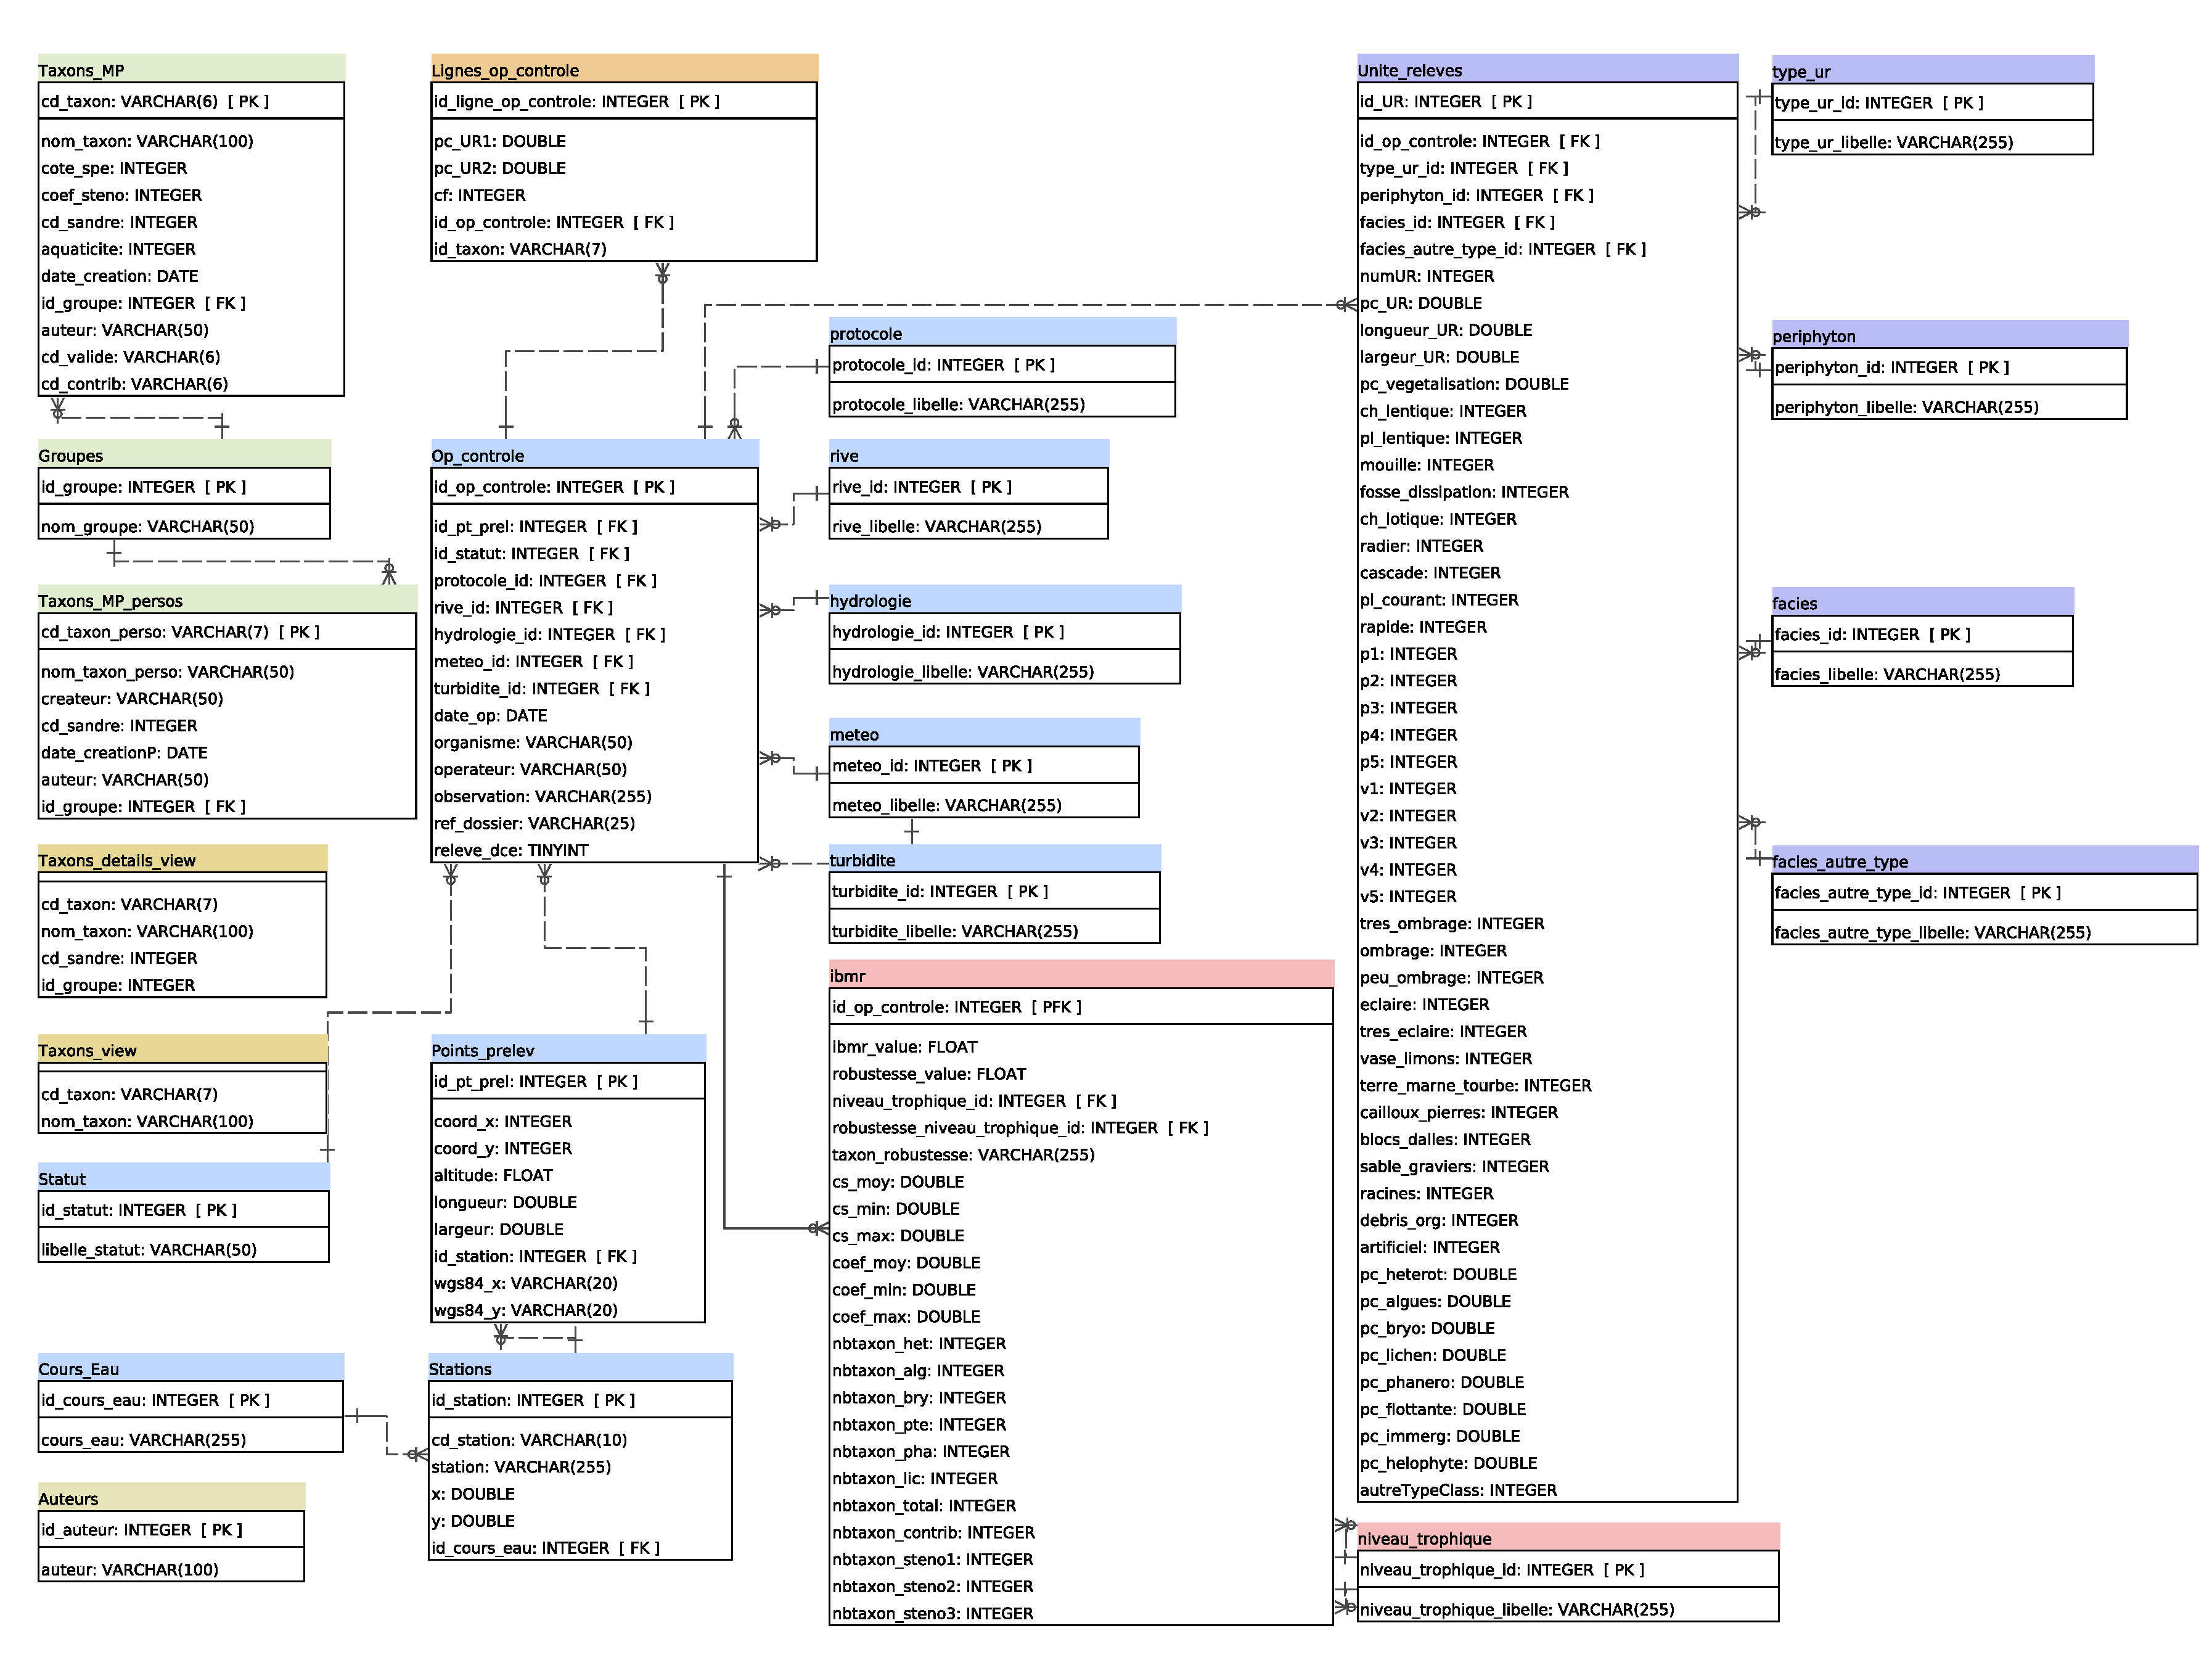
\includepdf[pages=-,scale=.8,pagecommand={}]{alisma_structure_db.pdf}
% \input{chapitre2}
% Table des matières
\tableofcontents
\end{document}
